\upaper{42}{Energy --- Mind and Matter}
\author{Mighty Messenger}
\vs p042 0:1 The foundation of the universe is material in the sense that energy is the basis of all existence, and pure energy is controlled by the Universal Father. Force, energy, is the one thing which stands as an everlasting monument demonstrating and proving the existence and presence of the Universal Absolute. This vast stream of energy proceeding from the Paradise Presences has never lapsed, never failed; there has never been a break in the infinite upholding.
\vs p042 0:2 The manipulation of universe energy is ever in accordance with the personal will and the all\hyp{}wise mandates of the Universal Father. This personal control of manifested power and circulating energy is modified by the co\hyp{}ordinate acts and decisions of the Eternal Son, as well as by the united purposes of the Son and the Father executed by the Conjoint Actor. These divine beings act personally and as individuals; they also function in the persons and powers of an almost unlimited number of subordinates, each variously expressive of the eternal and divine purpose in the universe of universes. But these functional and provisional modifications or transmutations of divine power in no way lessen the truth of the statement that all force\hyp{}energy is under the ultimate control of a personal God resident at the centre of all things.
\usection{1.\bibnobreakspace Paradise Forces and Energies}
\vs p042 1:1 The foundation of the universe is material, but the essence of life is spirit. The Father of spirits is also the ancestor of universes; the eternal Father of the Original Son is also the eternity\hyp{}source of the original pattern, the Isle of Paradise.
\vs p042 1:2 Matter --- energy --- for they are but diverse manifestations of the same cosmic reality, as a universe phenomenon is inherent in the Universal Father. “In him all things consist.” Matter may appear to manifest inherent energy and to exhibit self\hyp{}contained powers, but the lines of gravity involved in the energies concerned in all these physical phenomena are derived from, and are dependent on, Paradise. The ultimaton, the first measurable form of energy, has Paradise as its nucleus.
\vs p042 1:3 \pc There is innate in matter and present in universal space a form of energy not known on Urantia. When this discovery is finally made, then will physicists feel that they have solved, almost at least, the mystery of matter. And so will they have approached one step nearer the Creator; so will they have mastered one more phase of the divine technique; but in no sense will they have found God, neither will they have established the existence of matter or the operation of natural laws apart from the cosmic technique of Paradise and the motivating purpose of the Universal Father.
\vs p042 1:4 Subsequent to even still greater progress and further discoveries, after Urantia has advanced immeasurably in comparison with present knowledge, though you should gain control of the energy revolutions of the electrical units of matter to the extent of modifying their physical manifestations --- even after all such possible progress, forever will scientists be powerless to create one atom of matter or to originate one flash of energy or ever to add to matter that which we call life.
\vs p042 1:5 \pc The creation of energy and the bestowal of life are the prerogatives of the Universal Father and his associate Creator personalities. The river of energy and life is a continuous outpouring from the Deities, the universal and united stream of Paradise force going forth to all space. This divine energy pervades all creation. The force organizers initiate those changes and institute those modifications of space\hyp{}force which eventuate in energy; the power directors transmute energy into matter; thus the material worlds are born. The Life Carriers initiate those processes in dead matter which we call life, material life. The Morontia Power Supervisors likewise perform throughout the transition realms between the material and the spiritual worlds. The higher spirit Creators inaugurate similar processes in divine forms of energy, and there ensue the higher spirit forms of intelligent life.
\vs p042 1:6 \pc Energy proceeds from Paradise, fashioned after the divine order. Energy --- pure energy --- partakes of the nature of the divine organization; it is fashioned after the similitude of the three Gods embraced in one, as they function at the headquarters of the universe of universes. And all force is circuited in Paradise, comes from the Paradise Presences and returns thereto, and is in essence a manifestation of the uncaused Cause --- the Universal Father; and without the Father would not anything exist that does exist.
\vs p042 1:7 Force derived from self\hyp{}existent Deity is in itself ever existent. Force\hyp{}energy is imperishable, indestructible; these manifestations of the Infinite may be subject to unlimited transmutation, endless transformation, and eternal metamorphosis; but in no sense or degree, not even to the slightest imaginable extent, could they or ever shall they suffer extinction. But energy, though springing from the Infinite, is not infinitely manifest; there are outer limits to the presently conceived master universe.
\vs p042 1:8 Energy is eternal but not infinite; it ever responds to the all\hyp{}embracing grasp of Infinity. Forever force and energy go on; having gone out from Paradise, they must return thereto, even if age upon age be required for the completion of the ordained circuit. That which is of Paradise Deity origin can have only a Paradise destination or a Deity destiny.
\vs p042 1:9 \pc And all this confirms our belief in a circular, somewhat limited, but orderly and far\hyp{}flung universe of universes. If this were not true, then evidence of energy depletion at some point would sooner or later appear. All laws, organizations, administration, and the testimony of universe explorers --- everything points to the existence of an infinite God but, as yet, a finite universe, a circularity of endless existence, well\hyp{}nigh limitless but, nevertheless, finite in contrast with infinity.
\usection{2.\bibnobreakspace Universal Nonspiritual Energy Systems\\(\subtitlefont Physical Energies)}
\vs p042 2:1 It is indeed difficult to find suitable words in the English language whereby to designate and wherewith to describe the various levels of force and energy --- physical, mindal, or spiritual. These narratives cannot altogether follow your accepted definitions of force, energy, and power. There is such paucity of language that we must use these terms in multiple meanings. In this paper, for example, the word \bibemph{energy} is used to denote all phases and forms of phenomenal motion, action, and potential, while \bibemph{force} is applied to the pregravity, and \bibemph{power} to the postgravity, stages of energy.
\vs p042 2:2 I will, however, endeavour to lessen conceptual confusion by suggesting the advisability of adopting the following classification for cosmic force, emergent energy, and universe power --- physical energy:
\vs p042 2:3 \ublistelem{1.}\bibnobreakspace \bibemph{Space potency.} This is the unquestioned free space presence of the Unqualified Absolute. The extension of this concept connotes the universe force\hyp{}space potential inherent in the functional totality of the Unqualified Absolute, while the intension of this concept implies the totality of cosmic reality --- universes --- which emanated eternitywise from the never\hyp{}beginning, never\hyp{}ending, never\hyp{}moving, never\hyp{}changing Isle of Paradise.
\vs p042 2:4 The phenomena indigenous to the nether side of Paradise probably embrace three zones of absolute force presence and performance: the fulcral zone of the Unqualified Absolute, the zone of the Isle of Paradise itself, and the intervening zone of certain unidentified equalizing and compensating agencies or functions. These triconcentric zones are the centrum of the Paradise cycle of cosmic reality.
\vs p042 2:5 Space potency is a prereality; it is the domain of the Unqualified Absolute and is responsive only to the personal grasp of the Universal Father, notwithstanding that it is seemingly modifiable by the presence of the Primary Master Force Organizers.
\vs p042 2:6 On Uversa, space potency is spoken of as ABSOLUTA.
\vs p042 2:7 \ublistelem{2.}\bibnobreakspace \bibemph{Primordial force.} This represents the first basic change in space potency and may be one of the nether Paradise functions of the Unqualified Absolute. We know that the space presence going out from nether Paradise is modified in some manner from that which is incoming. But regardless of any such possible relationships, the openly recognized transmutation of space potency into primordial force is the primary differentiating function of the tension\hyp{}presence of the living Paradise force organizers.
\vs p042 2:8 Passive and potential force becomes active and primordial in response to the resistance afforded by the space presence of the Primary Eventuated Master Force Organizers. Force is now emerging from the exclusive domain of the Unqualified Absolute into the realms of multiple response --- response to certain primal motions initiated by the God of Action and thereupon to certain compensating motions emanating from the Universal Absolute. Primordial force is seemingly reactive to transcendental causation in proportion to absoluteness.
\vs p042 2:9 Primordial force is sometimes spoken of as \bibemph{pure energy;} on Uversa we refer to it as SEGREGATA.
\vs p042 2:10 \ublistelem{3.}\bibnobreakspace \bibemph{Emergent energies.} The passive presence of the primary force organizers is sufficient to transform space potency into primordial force, and it is upon such an activated space field that these same force organizers begin their initial and active operations. Primordial force is destined to pass through two distinct phases of transmutation in the realms of energy manifestation before appearing as universe power. These two levels of emerging energy are:
\vs p042 2:11 \ublistelem{a.}\bibnobreakspace \bibemph{Puissant energy.} This is the powerful\hyp{}directional, mass\hyp{}movemented, mighty\hyp{}tensioned, and forcible\hyp{}reacting energy --- gigantic energy systems set in motion by the activities of the primary force organizers. This primary or puissant energy is not at first definitely responsive to the Paradise\hyp{}gravity pull though probably yielding an aggregate\hyp{}mass or space\hyp{}directional response to the collective group of absolute influences operative from the nether side of Paradise. When energy emerges to the level of initial response to the circular and absolute\hyp{}gravity grasp of Paradise, the primary force organizers give way to the functioning of their secondary associates.
\vs p042 2:12 \ublistelem{b.}\bibnobreakspace \bibemph{Gravity energy.} The now\hyp{}appearing gravity\hyp{}responding energy carries the potential of universe power and becomes the active ancestor of all universe matter. This secondary or gravity energy is the product of the energy elaboration resulting from the pressure\hyp{}presence and the tension\hyp{}trends set up by the Associate Transcendental Master Force Organizers. In response to the work of these force manipulators, space\hyp{}energy rapidly passes from the puissant to the gravity stage, thus becoming directly responsive to the circular grasp of Paradise (absolute) gravity while disclosing a certain potential for sensitivity to the linear\hyp{}gravity pull inherent in the soon appearing material mass of the electronic and the postelectronic stages of energy and matter. Upon the appearance of gravity response, the Associate Master Force Organizers may retire from the energy cyclones of space provided the Universe Power Directors are assignable to that field of action.
\vs p042 2:13 \pc We are quite uncertain regarding the exact causes of the early stages of force evolution, but we recognize the intelligent action of the Ultimate in both levels of emergent\hyp{}energy manifestation. Puissant and gravity energies, when regarded collectively, are spoken of on Uversa as ULTIMATA.
\vs p042 2:14 \ublistelem{4.}\bibnobreakspace \bibemph{Universe power.} Space\hyp{}force has been changed into space\hyp{}energy and thence into the energy of gravity control. Thus has physical energy been ripened to that point where it can be directed into channels of power and made to serve the manifold purposes of the universe Creators. This work is carried on by the versatile directors, centres, and controllers of physical energy in the grand universe --- the organized and inhabited creations. These Universe Power Directors assume the more or less complete control of 21 of the 30 phases of energy constituting the present energy system of the 7 superuniverses. This domain of power\hyp{}energy\hyp{}matter is the realm of the intelligent activities of the Sevenfold, functioning under the time\hyp{}space overcontrol of the Supreme.
\vs p042 2:15 On Uversa we refer to the realm of universe power as GRAVITA.
\vs p042 2:16 \ublistelem{5.}\bibnobreakspace \bibemph{Havona energy.} In concept this narrative has been moving Paradiseward as transmuting space\hyp{}force has been followed, level by level, to the working level of the energy\hyp{}power of the universes of time and space. Continuing Paradiseward, there is next encountered a pre\hyp{}existent phase of energy which is characteristic of the central universe. Here the evolutionary cycle seems to turn back upon itself; energy\hyp{}power now seems to begin to swing back towards force, but force of a nature very unlike that of space potency and primordial force. Havona energy systems are not dual; they are triune. This is the existential energy domain of the Conjoint Actor, functioning in behalf of the Paradise Trinity.
\vs p042 2:17 On Uversa these energies of Havona are known as TRIATA.
\vs p042 2:18 \ublistelem{6.}\bibnobreakspace \bibemph{Transcendental energy.} This energy system operates on and from the upper level of Paradise and only in connection with the absonite peoples. On Uversa it is denominated TRANOSTA.
\vs p042 2:19 \ublistelem{7.}\bibnobreakspace \bibemph{Monota.} Energy is close of kin to divinity when it is Paradise energy. We incline to the belief that monota is the living, nonspirit energy of Paradise --- an eternity counterpart of the living, spirit energy of the Original Son --- hence the nonspiritual energy system of the Universal Father.
\vs p042 2:20 We cannot differentiate the \bibemph{nature} of Paradise spirit and Paradise monota; they are apparently alike. They have different names, but you can hardly be told very much about a reality whose spiritual and whose nonspiritual manifestations are distinguishable only by \bibemph{name.}
\vs p042 2:21 \pc We know that finite creatures can attain the worship experience of the Universal Father through the ministry of God the Sevenfold and the Thought Adjusters, but we doubt that any subabsolute personality, even power directors, can comprehend the energy infinity of the First Great Source and Centre. One thing is certain: If the power directors are conversant with the technique of the metamorphosis of space\hyp{}force, they do not reveal the secret to the rest of us. It is my opinion that they do not fully comprehend the function of the force organizers.
\vs p042 2:22 These power directors themselves are energy catalysers; that is, they cause energy to segment, organize, or assemble in unit formation by their presence. And all this implies that there must be something inherent in energy which causes it thus to function in the presence of these power entities. The Nebadon Melchizedeks long since denominated the phenomenon of the transmutation of cosmic force into universe power as one of the 7 “infinities of divinity.” And that is as far as you will advance on this point during your local universe ascension.
\vs p042 2:23 \pc Notwithstanding our inability fully to comprehend the origin, nature, and transmutations of cosmic force, we are fully conversant with all phases of emergent\hyp{}energy behaviour from the times of its direct and unmistakable response to the action of Paradise gravity --- about the time of the beginning of the function of the superuniverse power directors.
\usection{3.\bibnobreakspace Classification of Matter}
\vs p042 3:1 Matter in all universes, excepting in the central universe, is identical. Matter in its physical properties depends on the revolutionary rates of its component members, the number and size of the revolving members, their distance from the nuclear body or the space content of matter, as well as on the presence of certain forces as yet undiscovered on Urantia.
\vs p042 3:2 In the varied suns, planets, and space bodies there are 10 grand divisions of matter:
\vs p042 3:3 \ublistelem{1.}\bibnobreakspace Ultimatonic matter --- the prime physical units of material existence, the energy particles which go to make up electrons.
\vs p042 3:4 \ublistelem{2.}\bibnobreakspace Subelectronic matter --- the explosive and repellent stage of the solar supergases.
\vs p042 3:5 \ublistelem{3.}\bibnobreakspace Electronic matter --- the electrical stage of material differentiation --- electrons, protons, and various other units entering into the varied constitution of the electronic groups.
\vs p042 3:6 \ublistelem{4.}\bibnobreakspace Subatomic matter --- matter existing extensively in the interior of the hot suns.
\vs p042 3:7 \ublistelem{5.}\bibnobreakspace Shattered atoms --- found in the cooling suns and throughout space.
\vs p042 3:8 \ublistelem{6.}\bibnobreakspace Ionized matter --- individual atoms stripped of their outer (chemically active) electrons by electrical, thermal, or X\hyp{}ray activities and by solvents.
\vs p042 3:9 \ublistelem{7.}\bibnobreakspace Atomic matter --- the chemical stage of elemental organization, the component units of molecular or visible matter.
\vs p042 3:10 \ublistelem{8.}\bibnobreakspace The molecular stage of matter --- matter as it exists on Urantia in a state of relatively stable materialization under ordinary conditions.
\vs p042 3:11 \ublistelem{9.}\bibnobreakspace Radioactive matter --- the disorganizing tendency and activity of the heavier elements under conditions of moderate heat and diminished gravity pressure.
\vs p042 3:12 \ublistelem{10.}\bibnobreakspace Collapsed matter --- the relatively stationary matter found in the interior of the cold or dead suns. This form of matter is not really stationary; there is still some ultimatonic even electronic activity, but these units are in very close proximity, and their rates of revolution are greatly diminished.
\vs p042 3:13 \pc The foregoing classification of matter pertains to its organization rather than to the forms of its appearance to created beings. Neither does it take into account the pre\hyp{}emergent stages of energy nor the eternal materializations on Paradise and in the central universe.
\usection{4.\bibnobreakspace Energy and Matter Transmutations}
\vs p042 4:1 Light, heat, electricity, magnetism, chemism, energy, and matter are --- in origin, nature, and destiny --- one and the same thing, together with other material realities as yet undiscovered on Urantia.
\vs p042 4:2 We do not fully comprehend the almost endless changes to which physical energy may be subject. In one universe it appears as light, in another as light plus heat, in another as forms of energy unknown on Urantia; in untold millions of years it may reappear as some form of restless, surging electrical energy or magnetic power; and still later on it may again appear in a subsequent universe as some form of variable matter going through a series of metamorphoses, to be followed by its outward physical disappearance in some great cataclysm of the realms. And then, after countless ages and almost endless wandering through numberless universes, again may this same energy re\hyp{}emerge and many times change its form and potential; and so do these transformations continue through successive ages and throughout countless realms. Thus matter sweeps on, undergoing the transmutations of time but swinging ever true to the circle of eternity; even if long prevented from returning to its source, it is ever responsive thereto, and it ever proceeds in the path ordained by the Infinite Personality who sent it forth.
\vs p042 4:3 The power centres and their associates are much concerned in the work of transmuting the ultimaton into the circuits and revolutions of the electron. These unique beings control and compound power by their skillful manipulation of the basic units of materialized energy, the ultimatons. They are masters of energy as it circulates in this primitive state. In liaison with the physical controllers they are able to effectively control and direct energy even after it has transmuted to the electrical level, the so\hyp{}called electronic stage. But their range of action is enormously curtailed when electronically organized energy swings into the whirls of the atomic systems. Upon such materialization, these energies fall under the complete grasp of the drawing power of linear gravity.
\vs p042 4:4 Gravity acts positively on the power lanes and energy channels of the power centres and the physical controllers, but these beings have only a negative relation to gravity --- the exercise of their antigravity endowments.
\vs p042 4:5 Throughout all space, cold and other influences are at work creatively organizing ultimatons into electrons. Heat is the measurement of electronic activity, while cold merely signifies absence of heat --- comparative energy rest --- the status of the universal force\hyp{}charge of space provided neither emergent energy nor organized matter were present and responding to gravity.
\vs p042 4:6 Gravity presence and action is what prevents the appearance of the theoretical absolute zero, for interstellar space does not have the temperature of absolute zero. Throughout all organized space there are gravity\hyp{}responding energy currents, power circuits, and ultimatonic activities, as well as organizing electronic energies. Practically speaking, space is not empty. Even the atmosphere of Urantia thins out increasingly until at about 4,800\,km it begins to shade off into the average space matter in this section of the universe. The most nearly empty space known in Nebadon would yield about 100 ultimatons --- the equivalent of one electron --- in 16.4 cm\ts{3} . Such scarcity of matter is regarded as practically empty space.
\vs p042 4:7 Temperature --- heat and cold --- is secondary only to gravity in the realms of energy and matter evolution. Ultimatons are humbly obedient to temperature extremes. Low temperatures favour certain forms of electronic construction and atomic assembly, while high temperatures facilitate all sorts of atomic breakup and material disintegration.
\vs p042 4:8 When subjected to the heat and pressure of certain internal solar states, all but the most primitive associations of matter may be broken up. Heat can thus largely overcome gravity stability. But no known solar heat or pressure can convert ultimatons back into puissant energy.
\vs p042 4:9 The blazing suns can transform matter into various forms of energy, but the dark worlds and all outer space can slow down electronic and ultimatonic activity to the point of converting these energies into the matter of the realms. Certain electronic associations of a close nature, as well as many of the basic associations of nuclear matter, are formed in the exceedingly low temperatures of open space, being later augmented by association with larger accretions of materializing energy.
\vs p042 4:10 Throughout all of this never\hyp{}ending metamorphosis of energy and matter we must reckon with the influence of gravity pressure and with the antigravity behaviour of the ultimatonic energies under certain conditions of temperature, velocity, and revolution. Temperature, energy currents, distance, and the presence of the living force organizers and the power directors also have a bearing on all transmutation phenomena of energy and matter.
\vs p042 4:11 The increase of mass in matter is equal to the increase of energy divided by the square of the velocity of light. \begin{equation}\Delta m = {\Delta E \over c^2}\end{equation} In a dynamic sense the work which resting matter can perform is equal to the energy expended in bringing its parts together from Paradise minus the resistance of the forces overcome in transit and the attraction exerted by the parts of matter on one another.
\vs p042 4:12 \pc The existence of pre\hyp{}electronic forms of matter is indicated by the two atomic weights of lead. The lead of original formation weighs slightly more than that produced through uranium disintegration by way of radium emanations\fnst{\textbf{radium emanations}, the archaic term for the chemical element radon ($^{222}_{86}$Rn), which is the indirect decay product (via radium $^{226}_{88}$Ra) of Uranium-238.}; and this difference in atomic weight represents the actual loss of energy in the atomic breakup.\tunemarkup{pictures}{\begin{figure}[H]\centering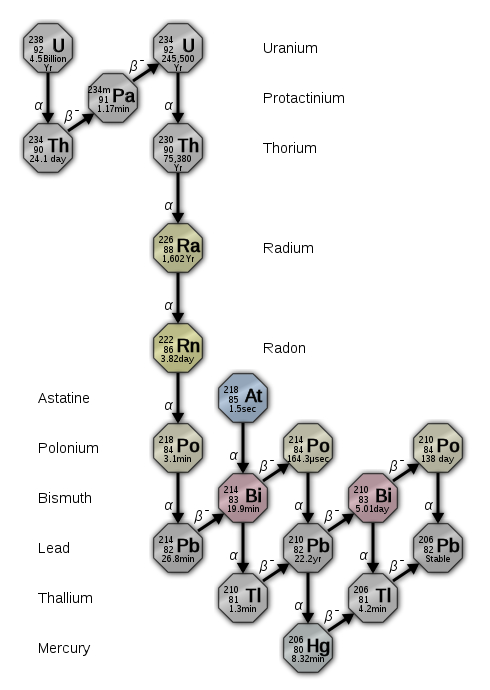
\includegraphics[width=\columnwidth]{../urantia-pictures/Uranium-Decay-Series.jpg}\caption{Uranium-238 decay series ending in Lead-206}\end{figure}}
\vs p042 4:13 \pc The relative integrity of matter is assured by the fact that energy can be absorbed or released only in those exact amounts which Urantia scientists have designated quanta. This wise provision in the material realms serves to maintain the universes as going concerns.
\vs p042 4:14 The quantity of energy taken in or given out when electronic or other positions are shifted is always a “quantum” or some multiple thereof, but the vibratory or wavelike behaviour of such units of energy is wholly determined by the dimensions of the material structures concerned. Such wavelike energy ripples are 860\fnst{\textbf{860}, This ``magic number'' is explained by Sir James Jeans in his book ``The Universe Around Us'' (1930, p.138) as follows: the energy needed to separate two charges $+e$ and $-e$ apart at a distance $r$ is $e^2/{4\pi\epsilon_0 r}$; equating it to the energy of photon $h\nu$ we have $h\nu=hc\lambda = e^2/{4\pi\epsilon_0 r}$, whence we obtain $\lambda/r = 4\pi\epsilon_0 hc/e^2 \approx 861.02$.} times the diameters of the ultimatons, electrons, atoms, or other units thus performing. The never\hyp{}ending confusion attending the observation of the wave mechanics of quantum behaviour is due to the superimposition of energy waves: Two crests can combine to make a double\hyp{}height crest, while a crest and a trough may combine, thus producing mutual cancellation.
\usection{5.\bibnobreakspace Wave\hyp{}Energy Manifestations}
\vs p042 5:1 In the superuniverse of Orvonton there are 100 octaves of wave energy. Of these 100 groups of energy manifestations, 64 are wholly or partially recognized on Urantia. The sun’s rays constitute 4 octaves in the superuniverse scale, the visible rays embracing a single octave, number 46\fnst{\textbf{the visible rays embracing a single octave, number 46}, The wavelength of the visible light ranges between 400\,nm and 780\,nm, therefore the base frequency used for calibrating the spectrum is 11\,Hz: $\nu_{max}(n) = 11 \times 2^n$, where $\nu_{max}$ is the top frequency (in Hz) of the $n^{th}$ octave.} in this series. The ultraviolet group comes next, while 10 octaves up are the X\hyp{}rays, followed by the γ-rays\fnc{\textbf{γ-rays}, 1955 text: \bibtextul{Y rays}.} of radium. 32 octaves above the visible light of the sun are the outer\hyp{}space energy rays so frequently commingled with their associated highly energized minute particles of matter. Next downward from visible sunlight appear the infrared rays, and 30 octaves below are the radio transmission group.
\vs p042 5:2 \pc Wavelike energy manifestations --- from the standpoint of XX century Urantia scientific enlightenment --- may be classified into the following 10 groups:
\vs p042 5:3 \ublistelem{1.}\bibnobreakspace \bibemph{Infraultimatonic rays ---} the borderland revolutions of ultimatons as they begin to assume definite form. This is the 1\ts{st} stage of emergent energy in which wavelike phenomena can be detected and measured.
\vs p042 5:4 \ublistelem{2.}\bibnobreakspace \bibemph{Ultimatonic rays.} The assembly of energy into the minute spheres of the ultimatons occasions vibrations in the content of space which are discernible and measurable. And long before physicists ever discover the ultimaton, they will undoubtedly detect the phenomena of these rays as they shower in upon Urantia. These short and powerful rays represent the initial activity of the ultimatons as they are slowed down to that point where they veer towards the electronic organization of matter. As the ultimatons aggregate into electrons, condensation occurs with a consequent storage of energy.
\vs p042 5:5 \ublistelem{3.}\bibnobreakspace \bibemph{The short space rays.} These are the shortest of all purely electronic vibrations and represent the preatomic stage of this form of matter. These rays require extraordinarily high or low temperatures for their production. There are two sorts of these space rays: one attendant upon the birth of atoms and the other indicative of atomic disruption. They emanate in the largest quantities from the densest plane of the superuniverse, the Milky Way, which is also the densest plane of the outer universes.
\vs p042 5:6 \ublistelem{4.}\bibnobreakspace \bibemph{The electronic stage.} This stage of energy is the basis of all materialization in the 7 superuniverses. When electrons pass from higher to lower energy levels of orbital revolution, quanta are always given off. Orbital shifting of electrons results in the ejection or the absorption of very definite and uniform measurable particles of light\hyp{}energy, while the individual electron always gives up a particle of light\hyp{}energy when subjected to collision. Wavelike energy manifestations also attend upon the performances of the positive bodies and the other members of the electronic stage.
\vs p042 5:7 \ublistelem{5.}\bibnobreakspace \bibemph{Gamma rays ---} those emanations which characterize the spontaneous dissociation of atomic matter. The best illustration of this form of electronic activity is in the phenomena associated with radium disintegration.
\vs p042 5:8 \ublistelem{6.}\bibnobreakspace \bibemph{The X\hyp{}ray group.} The next step in the slowing down of the electron yields the various forms of solar X\hyp{}rays together with artificially generated X\hyp{}rays. The electronic charge creates an electric field; movement gives rise to an electric current; the current produces a magnetic field. When an electron is suddenly stopped, the resultant electromagnetic commotion produces the X\hyp{}ray; the X\hyp{}ray is \bibemph{that} disturbance. The solar X\hyp{}rays are identical with those which are mechanically generated for exploring the interior of the human body except that they are a trifle longer.
\vs p042 5:9 \ublistelem{7.}\bibnobreakspace \bibemph{The ultraviolet} or chemical rays of sunlight and the various mechanical productions.
\vs p042 5:10 \ublistelem{8.}\bibnobreakspace \bibemph{The white light ---} the whole visible light of the suns.
\vs p042 5:11 \ublistelem{9.}\bibnobreakspace \bibemph{Infrared rays ---} the slowing down of electronic activity still nearer the stage of appreciable heat.
\vs p042 5:12 \ublistelem{10.}\bibnobreakspace \bibemph{Hertzian waves ---} those energies utilized on Urantia for broadcasting.
\vs p042 5:13 \pc Of all these 10 phases of wavelike energy activity, the human eye can react to just one octave, the whole light of ordinary sunlight.
\vs p042 5:14 \pc The so\hyp{}called ether is merely a collective name to designate a group of force and energy activities occurring in space. Ultimatons, electrons, and other mass aggregations of energy are uniform particles of matter, and in their transit through space they really proceed in direct lines. Light and all other forms of recognizable energy manifestations consist of a succession of definite energy particles which proceed in direct lines except as modified by gravity and other intervening forces. That these processions of energy particles appear as wave phenomena when subjected to certain observations is due to the resistance of the undifferentiated force blanket of all space, the hypothetical ether, and to the intergravity tension of the associated aggregations of matter. The spacing of the particle\hyp{}intervals of matter, together with the initial velocity of the energy beams, establishes the undulatory appearance of many forms of energy\hyp{}matter.
\vs p042 5:15 The excitation of the content of space produces a wavelike reaction to the passage of rapidly moving particles of matter, just as the passage of a ship through water initiates waves of varying amplitude and interval.
\vs p042 5:16 Primordial\hyp{}force behaviour does give rise to phenomena which are in many ways analogous to your postulated ether. Space is not empty; the spheres of all space whirl and plunge on through a vast ocean of outspread force\hyp{}energy; neither is the space content of an atom empty. Nevertheless there is no ether, and the very absence of this hypothetical ether enables the inhabited planet to escape falling into the sun and the encircling electron to resist falling into the nucleus.
\usection{6.\bibnobreakspace Ultimatons, Electrons, and Atoms}
\vs p042 6:1 While the space charge of universal force is homogeneous and undifferentiated, the organization of evolved energy into matter entails the concentration of energy into discrete masses of definite dimensions and established weight --- precise gravity reaction.
\vs p042 6:2 Local or linear gravity becomes fully operative with the appearance of the atomic organization of matter. Preatomic matter becomes slightly gravity responsive when activated by X\hyp{}ray and other similar energies, but no measurable linear\hyp{}gravity pull is exerted on free, unattached, and uncharged electronic\hyp{}energy particles or on unassociated ultimatons.
\vs p042 6:3 \pc Ultimatons function by mutual attraction, responding only to the circular Paradise\hyp{}gravity pull. Without linear\hyp{}gravity response they are thus held in the universal space drift. Ultimatons are capable of accelerating revolutionary velocity to the point of partial antigravity behaviour, but they cannot, independent of force organizers or power directors, attain the critical escape velocity of deindividuation, return to the puissant\hyp{}energy stage. In nature, ultimatons escape the status of physical existence only when participating in the terminal disruption of a cooled\hyp{}off and dying sun.
\vs p042 6:4 \pc The ultimatons, unknown on Urantia, slow down through many phases of physical activity before they attain the revolutionary\hyp{}energy prerequisites to electronic organization. Ultimatons have three varieties of motion: mutual resistance to cosmic force, individual revolutions of antigravity potential, and the intraelectronic positions of the 100 mutually interassociated ultimatons.
\vs p042 6:5 Mutual attraction holds 100 ultimatons together in the constitution of the electron; and there are never more nor less than 100 ultimatons in a typical electron. The loss of one or more ultimatons destroys typical electronic identity, thus bringing into existence one of the 10 modified forms of the electron.
\vs p042 6:6 Ultimatons do not describe orbits or whirl about in circuits within the electrons, but they do spread or cluster in accordance with their axial revolutionary velocities, thus determining the differential electronic dimensions. This same ultimatonic velocity of axial revolution also determines the negative or positive reactions of the several types of electronic units. The entire segregation and grouping of electronic matter, together with the electric differentiation of negative and positive bodies of energy\hyp{}matter, result from these various functions of the component ultimatonic interassociation.
\vs p042 6:7 \pc Each atom is a trifle over $2.54 \times 10^{-8}$ cm in diameter, while an electron weighs a little less than 1/2,000\ts{th} of the smallest atom, hydrogen. The positive proton, characteristic of the atomic nucleus, while it may be no larger than a negative electron, weighs from 2,000 to 3,000 times more.
\vs p042 6:8 \pc If the mass of matter should be magnified until that of an electron equalled 3\,g, then were size to be proportionately magnified, the volume of such an electron would become as large as that of the earth. If the volume of a proton --- 1,800 times as heavy as an electron --- should be magnified to the size of the head of a pin, then, in comparison, a pin’s head would attain a diameter equal to that of the earth’s orbit around the sun.
\usection{7.\bibnobreakspace Atomic Matter}
\vs p042 7:1 The formation of all matter is on the order of the solar system. There is at the centre of every minute universe of energy a relatively stable, comparatively stationary, nuclear portion of material existence. This central unit is endowed with a threefold possibility of manifestation. Surrounding this energy centre there whirl, in endless profusion but in fluctuating circuits, the energy units which are faintly comparable to the planets encircling the sun of some starry group like your own solar system.
\vs p042 7:2 \pc Within the atom the electrons revolve about the central proton with about the same comparative room the planets have as they revolve about the sun in the space of the solar system. There is the same relative distance, in comparison with actual size, between the atomic nucleus and the inner electronic circuit as exists between the inner planet, Mercury, and your sun.
\vs p042 7:3 The electronic axial revolutions and their orbital velocities about the atomic nucleus are both beyond the human imagination, not to mention the velocities of their component ultimatons. The positive particles of radium fly off into space at the rate of 16,000 km/s, while the negative particles attain a velocity approximating that of light.
\vs p042 7:4 \pc The local universes are of decimal construction. There are just 100 distinguishable atomic materializations of space\hyp{}energy in a dual universe; that is the maximum possible organization of matter in Nebadon. These 100 forms of matter consist of a regular series in which from 1 to 100 electrons revolve around a central and relatively compact nucleus. It is this orderly and dependable association of various energies that constitutes matter.
\vs p042 7:5 Not every world will show 100 recognizable elements at the surface, but they are somewhere present, have been present, or are in process of evolution. Conditions surrounding the origin and subsequent evolution of a planet determine how many of the 100 atomic types will be observable. The heavier atoms are not found on the surface of many worlds. Even on Urantia the known heavier elements manifest a tendency to fly to pieces, as is illustrated by radium behaviour.
\vs p042 7:6 Stability of the atom depends on the number of electrically inactive neutrons in the central body. Chemical behaviour is wholly dependent on the activity of the freely revolving electrons.
\vs p042 7:7 \pc In Orvonton it has never been possible naturally to assemble over 100 orbital electrons in one atomic system. When 101 have been artificially introduced into the orbital field, the result has always been the instantaneous disruption of the central proton with the wild dispersion of the electrons and other liberated energies.
\vs p042 7:8 \pc While atoms may contain from 1 to 100 orbital electrons, only the outer 10 electrons of the larger atoms revolve about the central nucleus as distinct and discrete bodies, intactly and compactly swinging around on precise and definite orbits. The 30 electrons nearest the centre are difficult of observation or detection as separate and organized bodies. This same comparative ratio of electronic behaviour in relation to nuclear proximity obtains in all atoms regardless of the number of electrons embraced. The nearer the nucleus, the less there is of electronic individuality. The wavelike energy extension of an electron may so spread out as to occupy the whole of the lesser atomic orbits; especially is this true of the electrons nearest the atomic nucleus.
\vs p042 7:9 The 30 innermost orbital electrons have individuality, but their energy systems tend to intermingle, extending from electron to electron and well\hyp{}nigh from orbit to orbit. The next 30 electrons constitute the second family, or energy zone, and are of advancing individuality, bodies of matter exerting a more complete control over their attendant energy systems. The next 30 electrons, the third energy zone, are still more individualized and circulate in more distinct and definite orbits. The last 10 electrons, present in only the 10 heaviest elements, are possessed of the dignity of independence and are, therefore, able to escape more or less freely from the control of the mother nucleus. With a minimum variation in temperature and pressure, the members of this fourth and outermost group of electrons will escape from the grasp of the central nucleus, as is illustrated by the spontaneous disruption of uranium and kindred elements.
\vs p042 7:10 The first 27 atoms, those containing from 1 to 27 orbital electrons, are more easy of comprehension than the rest. From 28 upward we encounter more and more of the unpredictability of the supposed presence of the Unqualified Absolute. But some of this electronic unpredictability is due to differential ultimatonic axial revolutionary velocities and to the unexplained “huddling” proclivity of ultimatons. Other influences --- physical, electrical, magnetic, and gravitational --- also operate to produce variable electronic behaviour. Atoms therefore are similar to persons as to predictability. Statisticians may announce laws governing a large number of either atoms or persons but not for a single individual atom or person.
\usection{8.\bibnobreakspace Atomic Cohesion}
\vs p042 8:1 While gravity is one of several factors concerned in holding together a tiny atomic energy system, there is also present in and among these basic physical units a powerful and unknown energy, the secret of their basic constitution and ultimate behaviour, a force which remains to be discovered on Urantia. This universal influence permeates all the space embraced within this tiny energy organization.
\vs p042 8:2 The interelectronic space of an atom is not empty. Throughout an atom this interelectronic space is activated by wavelike manifestations which are perfectly synchronized with electronic velocity and ultimatonic revolutions. This force is not wholly dominated by your recognized laws of positive and negative attraction; its behaviour is therefore sometimes unpredictable. This unnamed influence seems to be a space\hyp{}force reaction of the Unqualified Absolute.
\vs p042 8:3 \pc The charged protons and the uncharged neutrons of the nucleus of the atom are held together by the reciprocating function of the mesotron\fnst{mesotron --- nowadays called \emph{meson}. In particular, the $\pi^+$-meson (pion) here referred to is now (2012\,A.D.) considered to be 273 times as heavy as the electron.}, a particle of matter 180 times as heavy as the electron. Without this arrangement the electric charge carried by the protons would be disruptive of the atomic nucleus.
\vs p042 8:4 As atoms are constituted, neither electric nor gravitational forces could hold the nucleus together. The integrity of the nucleus is maintained by the reciprocal cohering function of the mesotron, which is able to hold charged and uncharged particles together because of superior force\hyp{}mass power and by the further function of causing protons and neutrons constantly to change places. The mesotron causes the electric charge of the nuclear particles to be incessantly tossed back and forth between protons and neutrons. At one infinitesimal part of a second a given nuclear particle is a charged proton and the next an uncharged neutron. And these alternations of energy status are so unbelievably rapid that the electric charge is deprived of all opportunity to function as a disruptive influence. Thus does the mesotron function as an “energy\hyp{}carrier” particle which mightily contributes to the nuclear stability of the atom\fnst{The mechanism of $\pi^+$ pion exchange described here was first suggested by Hideki Yukawa in 1935 and experimentally confirmed in 1947. Having \bibemph{finite mass} for the virtual quantum of strong field ideally corresponded to the fact that this interaction has a \bibemph{short} range, unlike the electromagnetic interaction explained by the \bibemph{massless} virtual photons. However, in 1964 it was superseded by the quark model, according to which the proton-neutron force is a kind of ``residual'' force caused by the gluon exchange between the quark constituents of nucleons. In the quark model, pions are thought to consist of quark-antiquark pairs (e.g. $\pi^+ = u\overline{d}$), just like all other mesons and so their \bibemph{special} role as the field quanta disappears.}.
\vs p042 8:5 The presence and function of the mesotron also explains another atomic riddle. When atoms perform radioactively, they emit far more energy than would be expected. This excess of radiation is derived from the breaking up of the mesotron “energy carrier,” which thereby becomes a mere electron. The mesotronic disintegration is also accompanied by the emission of certain small uncharged particles.
\vs p042 8:6 The mesotron explains certain cohesive properties of the atomic nucleus, but it does not account for the cohesion of proton to proton nor for the adhesion of neutron to neutron. The paradoxical and powerful force of atomic cohesive integrity is a form of energy as yet undiscovered on Urantia.
\vs p042 8:7 These mesotrons are found abundantly in the space rays which so incessantly impinge upon your planet.
\usection{9.\bibnobreakspace Natural Philosophy}
\vs p042 9:1 Religion is not alone dogmatic; natural philosophy equally tends to dogmatize. When a renowned religious teacher reasoned that the number 7 was fundamental to nature because there are 7 openings in the human head, if he had known more of chemistry, he might have advocated such a belief founded on a true phenomenon of the physical world. There is in all the physical universes of time and space, notwithstanding the universal manifestation of the decimal constitution of energy, the ever\hyp{}present reminder of the reality of the sevenfold electronic organization of prematter.
\vs p042 9:2 The number 7 is basic to the central universe and the spiritual system of inherent transmissions of character, but the number 10, the decimal system, is inherent in energy, matter, and the material creation. Nevertheless the atomic world does display a certain periodic characterization which recurs in groups of 7 --- a birthmark carried by this material world indicative of its far\hyp{}distant spiritual origin.
\vs p042 9:3 This sevenfold persistence of creative constitution is exhibited in the chemical domains as a recurrence of similar physical and chemical properties in segregated periods of 7 when the basic elements are arranged in the order of their atomic weights. When the Urantia chemical elements are thus arranged in a row, any given quality or property tends to recur by sevens. This periodic change by sevens recurs diminishingly and with variations throughout the entire chemical table, being most markedly observable in the earlier or lighter atomic groupings. Starting from any one element, after noting some one property, such a quality will change for six consecutive elements, but on reaching the eighth, it tends to reappear, that is, the eighth chemically active element resembles the first, the ninth the second, and so on. Such a fact of the physical world unmistakably points to the sevenfold constitution of ancestral energy and is indicative of the fundamental reality of the sevenfold diversity of the creations of time and space. Man should also note that there are 7 colours in the natural spectrum.
\vs p042 9:4 But not all the suppositions of natural philosophy are valid; for example, the hypothetical ether, which represents an ingenious attempt of man to unify his ignorance of space phenomena. The philosophy of the universe cannot be predicated on the observations of so\hyp{}called science. If such a metamorphosis could not be seen, a scientist would be inclined to deny the possibility of developing a butterfly out of a caterpillar.
\vs p042 9:5 Physical stability associated with biologic elasticity is present in nature only because of the well\hyp{}nigh infinite wisdom possessed by the Master Architects of creation. Nothing less than transcendental wisdom could ever design units of matter which are at the same time so stable and so efficiently flexible.
\usection{10.\bibnobreakspace Universal Nonspiritual Energy Systems\\(\subtitlefont Material Mind Systems)}
\vs p042 10:1 The endless sweep of relative cosmic reality,\fnc{cosmic \bibtextul{reality} from \ldots\ \bibexpl{Comma inserted.}} from the absoluteness of Paradise monota to the absoluteness of space potency, is suggestive of certain evolutions of relationship in the nonspiritual realities of the First Source and Centre --- those realities which are concealed in space potency, revealed in monota, and provisionally disclosed on intervening cosmic levels. This eternal cycle of energy, being circuited in the Father of universes, is absolute and, being absolute, is expansile in neither fact nor value; nevertheless the Primal Father is even now --- as always --- self\hyp{}realizing of an ever\hyp{}expanding arena of time\hyp{}space, and of time\hyp{}space\hyp{}transcended, meanings, an arena of changing relationships wherein energy\hyp{}matter is being progressively subjected to the overcontrol of living and divine spirit through the experiential striving of living and personal mind.
\vs p042 10:2 The universal nonspiritual energies are reassociated in the living systems of non\hyp{}Creator minds on various levels, certain of which may be depicted as follows:
\vs p042 10:3 \ublistelem{1.}\bibnobreakspace \bibemph{Preadjutant\hyp{}spirit minds.} This level of mind is nonexperiencing and on the inhabited worlds is ministered by the Master Physical Controllers. This is mechanical mind, the nonteachable intellect of the most primitive forms of material life, but the nonteachable mind functions on many levels beside that of primitive planetary life.
\vs p042 10:4 \ublistelem{2.}\bibnobreakspace \bibemph{Adjutant\hyp{}spirit minds.} This is the ministry of a local universe Mother Spirit functioning through her 7 adjutant mind\hyp{}spirits on the teachable (nonmechanical) level of material mind. On this level material mind is experiencing: as subhuman (animal) intellect in the first 5 adjutants; as human (moral) intellect in the 7 adjutants; as superhuman (midwayer) intellect in the last 2 adjutants.
\vs p042 10:5 \ublistelem{3.}\bibnobreakspace \bibemph{Evolving morontia minds ---} the expanding consciousness of evolving personalities in the local universe ascending careers. This is the bestowal of the local universe Mother Spirit in liaison with the Creator Son. This mind level connotes the organization of the morontia type of life vehicle, a synthesis of the material and the spiritual which is effected by the Morontia Power Supervisors of a local universe. Morontia mind functions differentially in response to the 570 levels of morontia life, disclosing increasing associative capacity with the cosmic mind on the higher levels of attainment. This is the evolutionary course of mortal creatures, but mind of a nonmorontia order is also bestowed by a Universe Son and a Universe Spirit upon the nonmorontia children of the local creations.
\vs p042 10:6 \pc \bibemph{The cosmic mind.} This is the sevenfold diversified mind of time and space, one phase of which is ministered by each of the Seven Master Spirits to one of the 7 superuniverses. The cosmic mind encompasses all finite\hyp{}mind levels and co\hyp{}ordinates experientially with the evolutionary\hyp{}deity levels of the Supreme Mind and transcendentally with the existential levels of absolute mind --- the direct circuits of the Conjoint Actor.
\vs p042 10:7 On Paradise, mind is absolute; in Havona, absonite; in Orvonton, finite. Mind always connotes the presence\hyp{}activity of living ministry plus varied energy systems, and this is true of all levels and of all kinds of mind. But beyond the cosmic mind it becomes increasingly difficult to portray the relationships of mind to nonspiritual energy. Havona mind is subabsolute but superevolutionary; being existential\hyp{}experiential, it is nearer the absonite than any other concept revealed to you. Paradise mind is beyond human understanding; it is existential, nonspatial, and nontemporal. Nevertheless, all of these levels of mind are overshadowed by the universal presence of the Conjoint Actor --- by the mind\hyp{}gravity grasp of the God of mind on Paradise.
\usection{11.\bibnobreakspace Universe Mechanisms}
\vs p042 11:1 In the evaluation and recognition of mind it should be remembered that the universe is neither mechanical nor magical; it is a creation of mind and a mechanism of law. But while in practical application the laws of nature operate in what seems to be the dual realms of the physical and the spiritual, in reality they are one. The First Source and Centre is the primal cause of all materialization and at the same time the first and final Father of all spirits. The Paradise Father appears personally in the extra\hyp{}Havona universes only as pure energy and pure spirit --- as the Thought Adjusters and other similar fragmentations.
\vs p042 11:2 \pc Mechanisms do not absolutely dominate the total creation; the universe of universes \bibemph{in toto} is mind planned, mind made, and mind administered. But the divine mechanism of the universe of universes is altogether too perfect for the scientific methods of the finite mind of man to discern even a trace of the dominance of the infinite mind. For this creating, controlling, and upholding mind is neither material mind nor creature mind; it is spirit\hyp{}mind functioning on and from creator levels of divine reality.
\vs p042 11:3 The ability to discern and discover mind in universe mechanisms depends entirely on the ability, scope, and capacity of the investigating mind engaged in such a task of observation. Time\hyp{}space minds, organized out of the energies of time and space, are subject to the mechanisms of time and space.
\vs p042 11:4 \pc Motion and universe gravitation are twin facets of the impersonal time\hyp{}space mechanism of the universe of universes. The levels of gravity response for spirit, mind, and matter are quite independent of time, but only true spirit levels of reality are independent of space (nonspatial). The higher mind levels of the universe --- the spirit\hyp{}mind levels --- may also be nonspatial, but the levels of material mind, such as human mind, are responsive to the interactions of universe gravitation, losing this response only in proportion to spirit identification. Spirit\hyp{}reality levels are recognized by their spirit content, and spirituality in time and space is measured inversely to the linear\hyp{}gravity response.
\vs p042 11:5 Linear\hyp{}gravity response is a quantitative measure of nonspirit energy. All mass --- organized energy --- is subject to this grasp except as motion and mind act upon it. Linear gravity is the short\hyp{}range cohesive force of the macrocosmos somewhat as the forces of intra\hyp{}atomic cohesion are the short\hyp{}range forces of the microcosmos. Physical materialized energy, organized as so\hyp{}called matter, cannot traverse space without affecting linear\hyp{}gravity response. Although such gravity response is directly proportional to mass, it is so modified by intervening space that the final result is no more than roughly approximated when expressed as inversely according to the square of the distance. Space eventually conquers linear gravitation because of the presence therein of the antigravity influences of numerous supermaterial forces which operate to neutralize gravity action and all responses thereto.
\vs p042 11:6 \pc Extremely complex and highly automatic\hyp{}appearing cosmic mechanisms always tend to conceal the presence of the originative or creative indwelling mind from any and all intelligences very far below the universe levels of the nature and capacity of the mechanism itself. Therefore is it inevitable that the higher universe mechanisms must appear to be mindless to the lower orders of creatures. The only possible exception to such a conclusion would be the implication of mindedness in the amazing phenomenon of an \bibemph{apparently self\hyp{}maintaining universe ---} but that is a matter of philosophy rather than one of actual experience.
\vs p042 11:7 Since mind co\hyp{}ordinates the universe, fixity of mechanisms is nonexistent. The phenomenon of progressive evolution associated with cosmic self\hyp{}maintenance is universal. The evolutionary capacity of the universe is inexhaustible in the infinity of spontaneity. Progress towards harmonious unity, a growing experiential synthesis superimposed on an ever\hyp{}increasing complexity of relationships, could be effected only by a purposive and dominant mind.
\vs p042 11:8 The higher the universe mind associated with any universe phenomenon, the more difficult it is for the lower types of mind to discover it. And since the mind of the universe mechanism is creative spirit\hyp{}mind (even the mindedness of the Infinite), it can never be discovered or discerned by the lower\hyp{}level minds of the universe, much less by the \bibemph{lowest} mind of all, the human. The evolving animal mind, while naturally God\hyp{}seeking, is not alone and of itself inherently God\hyp{}knowing.
\usection{12.\bibnobreakspace Pattern and Form --- Mind Dominance}
\vs p042 12:1 The evolution of mechanisms implies and indicates the concealed presence and dominance of creative mind. The ability of the mortal intellect to conceive, design, and create automatic mechanisms demonstrates the superior, creative, and purposive qualities of man’s mind as the dominant influence on the planet. Mind always reaches out towards:
\vs p042 12:2 \ublistelem{1.}\bibnobreakspace Creation of material mechanisms.
\vs p042 12:3 \ublistelem{2.}\bibnobreakspace Discovery of hidden mysteries.
\vs p042 12:4 \ublistelem{3.}\bibnobreakspace Exploration of remote situations.
\vs p042 12:5 \ublistelem{4.}\bibnobreakspace Formulation of mental systems.
\vs p042 12:6 \ublistelem{5.}\bibnobreakspace Attainment of wisdom goals.
\vs p042 12:7 \ublistelem{6.}\bibnobreakspace Achievement of spirit levels.
\vs p042 12:8 \ublistelem{7.}\bibnobreakspace The accomplishment of divine destinies --- supreme, ultimate, and absolute.
\vs p042 12:9 \pc Mind is always creative. The mind endowment of an individual animal, mortal, morontian, spirit ascender, or finality attainer is always competent to produce a suitable and serviceable body for the living creature identity. But the presence phenomenon of a personality or the pattern of an identity, as such, is not a manifestation of energy, either physical, mindal, or spiritual. The personality form is the \bibemph{pattern} aspect of a living being; it connotes the \bibemph{arrangement} of energies, and this, plus life and motion, is the \bibemph{mechanism} of creature existence.
\vs p042 12:10 Even spirit beings have form, and these spirit forms (patterns) are real. Even the highest type of spirit personalities have forms --- personality presences in every sense analogous to Urantia mortal bodies. Nearly all beings encountered in the 7 superuniverses are possessed of forms. But there are a few exceptions to this general rule: Thought Adjusters appear to be without form until after fusion with the surviving souls of their mortal associates. Solitary Messengers, Inspired Trinity Spirits, Personal Aids of the Infinite Spirit, Gravity Messengers, Transcendental Recorders, and certain others are also without discoverable form. But these are typical of the exceptional few; the great majority have bona fide personality forms, forms which are individually characteristic, and which are recognizable and personally distinguishable.
\vs p042 12:11 The liaison of the cosmic mind and the ministry of the adjutant mind\hyp{}spirits evolve a suitable physical tabernacle for the evolving human being. Likewise does the morontia mind individualize the morontia form for all mortal survivors. As the mortal body is personal and characteristic for every human being, so will the morontia form be highly individual and adequately characteristic of the creative mind which dominates it. No two morontia forms are any more alike than any two human bodies. The Morontia Power Supervisors sponsor, and the attending seraphim provide, the undifferentiated morontia material wherewith the morontia life can begin to work. And after the morontia life it will be found that spirit forms are equally diverse, personal, and characteristic of their respective spirit\hyp{}mind indwellers.
\vs p042 12:12 \pc On a material world you think of a body as having a spirit, but we regard the spirit as having a body. The material eyes are truly the windows of the spirit\hyp{}born soul. The spirit is the architect, the mind is the builder, the body is the material building.
\vs p042 12:13 \pc Physical, spiritual, and mindal energies, as such and in their pure states, do not fully interact as actuals of the phenomenal universes. On Paradise the three energies are co\hyp{}ordinate, in Havona co\hyp{}ordinated, while in the universe levels of finite activities there must be encountered all ranges of material, mindal, and spiritual dominance. In nonpersonal situations of time and space, physical energy seems to predominate, but it also appears that the more nearly spirit\hyp{}mind function approaches divinity of purpose and supremacy of action, the more nearly does the spirit phase become dominant; that on the ultimate level spirit\hyp{}mind may become all but completely dominant. On the absolute level spirit certainly is dominant. And from there on out through the realms of time and space, wherever a divine spirit reality is present, whenever a real spirit\hyp{}mind is functioning, there always tends to be produced a material or physical counterpart of that spirit reality.
\vs p042 12:14 The spirit is the creative reality; the physical counterpart is the time\hyp{}space reflection of the spirit reality, the physical repercussion of the creative action of spirit\hyp{}mind.
\vs p042 12:15 Mind universally dominates matter, even as it is in turn responsive to the ultimate overcontrol of spirit. And with mortal man, only that mind which freely submits itself to the spirit direction can hope to survive the mortal time\hyp{}space existence as an immortal child of the eternal spirit world of the Supreme, the Ultimate, and the Absolute: the Infinite.
\vsetoff
\vs p042 12:16 [Presented by a Mighty Messenger on duty in Nebadon and by the request of Gabriel.]
\quizlink
